\documentclass{standalone}
\usepackage{tikz}
\usepackage{ctex,siunitx,ninecolors}
\setCJKmainfont{Noto Serif CJK SC}
\usepackage{tkz-euclide}
\usepackage{amsmath}
\usepackage{wasysym}
\usetikzlibrary{patterns, calc}
\usetikzlibrary {decorations.pathmorphing, decorations.pathreplacing, decorations.shapes}
\newcommand{\posthead}[2][gray]{
  \begin{scope}[#2]
    \fill[left color=#1,right color= #1,middle color=#1!20](0,0)ellipse(0.05 and 0.02);
    \fill[left color=#1,right color= #1,middle color=#1!20](0.05,0)rectangle(-0.05,0.07);
    \fill[left color=#1,right color= #1,middle color=#1!20](-0.06,0.07)arc(-180:0:0.06 and 0.02)--(0.06,0.15)--(0.05,0.16)--(-0.05,0.16)--(-0.06,0.15)--cycle;
    \fill[#1!50!gray](0,0.16)ellipse(0.05 and 0.02);
    \foreach \x in {75,45,15,-15,-45,-75}
    {
      \draw[very thin,#1!50!gray]({0.05*sin(\x)},{0.16-0.02*cos(\x)})--({0.06*sin(\x)},{0.15-0.02*cos(\x)})--++(0,-0.08);
    }
  \end{scope}
}
\begin{document}
\small
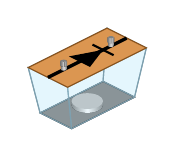
\begin{tikzpicture}[>=latex,scale=1.0]
  \draw[fill=gray](-0.2,-0.3)--(-0.6,-0.1)--(0.2,0.3)--(0.6,0.1)--cycle;
  \fill[left color=gray,right color=gray,middle color=white](0,0)ellipse(0.2 and 0.1);
  \fill[left color=gray,right color=gray,middle color=white](-0.2,0)rectangle(0.2,0.05);
  \fill[lightgray](0,0.05)ellipse(0.2 and 0.1);
  \draw[cyan!30!gray,fill=cyan!30,fill opacity=0.2](-0.60,-0.1)--(-0.75,0.475)--(-0.25,0.225)--(-0.2,-0.3)--cycle;
  \draw[cyan!30!gray,fill=cyan!30,fill opacity=0.2](-0.25,0.225)--(0.75,0.725)--(0.6,0.1)--(-0.2,-0.3)--cycle;
  \draw[cyan!30!gray,fill=cyan!30,fill opacity=0.2](0.25,0.975)--(0.75,0.725)--(0.6,0.1)--(0.2,0.3)--cycle;
  \draw[cyan!30!gray,fill=cyan!30,fill opacity=0.2](0.25,0.975)--(-0.75,0.475)--(-0.60,-0.1)--(0.2,0.3)--cycle;
  \draw[brown4,fill=brown7](0.25,0.975)--(-0.75,0.475)--(-0.25,0.225)--(0.75,0.725)--cycle;
  \draw[very thick] (-0.5,0.35)--(0.5,0.85);
  \fill(0.2,0.7)--(-0.2342,0.6171)--(0.0342,0.4829)--cycle;
  \draw[thick] (0.0658,0.7671)--(0.3342,0.6329);
  \posthead{xshift=-3mm,yshift=4.5mm,scale=0.7}
  \posthead{xshift=3mm,yshift=7.5mm,scale=0.7}
\end{tikzpicture}
\end{document}